\documentclass[12pt,letter]{article}
\usepackage[moduleName={Fourier},version={1.0.0}]{ArhythmeticUnits}

\begin{document}
\titlePage{img/Logo}{img/Module}{img/ArhythmeticUnits}

% ----------------------------------------------------------------------------
% MARK: Overview
% ----------------------------------------------------------------------------

\section{Overview}

% \begin{picture}(0,0)
%   \put(\paperwidth - 275,-\paperheight + 125){%
%     
\includegraphics[width=0.3\paperwidth]{img/Tag1}%
%   }
% \end{picture}

Jean-Baptiste Joseph Fourier (see Fig.~\ref{fig:fourier-portrait}) showed
that complex signals can be decomposed into sums of simpler trigonometric
functions. \textbf{Fourier} brings this concept to the virtual Eurorack
form-factor with deep control over the analysis parameters. Key features
include:
\begin{itemize}
  \item \textbf{Fully Parametric STFT:} Enjoy complete control over FFT
  length, hop size, and window function parameters, enabling precise tuning
  for a wide range of musical and engineering applications.
  \item \textbf{Time \& Frequency Smoothing:} Apply smoothing in both the
  temporal and spectral domains to consolidate FFT coefficients, thereby
  highlighting overarching trends in signal frequency content.
  \item \textbf{Slope Scaling:} Compensate for the natural roll-off of
  high-frequency energy, yielding a frequency representation that more
  accurately reflects human auditory perception.
  \item \textbf{Intuitive Interface:} A streamlined control layout delivers
  deep functionality without the need for extensive menu diving or manual
  exploration.
\end{itemize}

\begin{figure}[!htp]
\centering
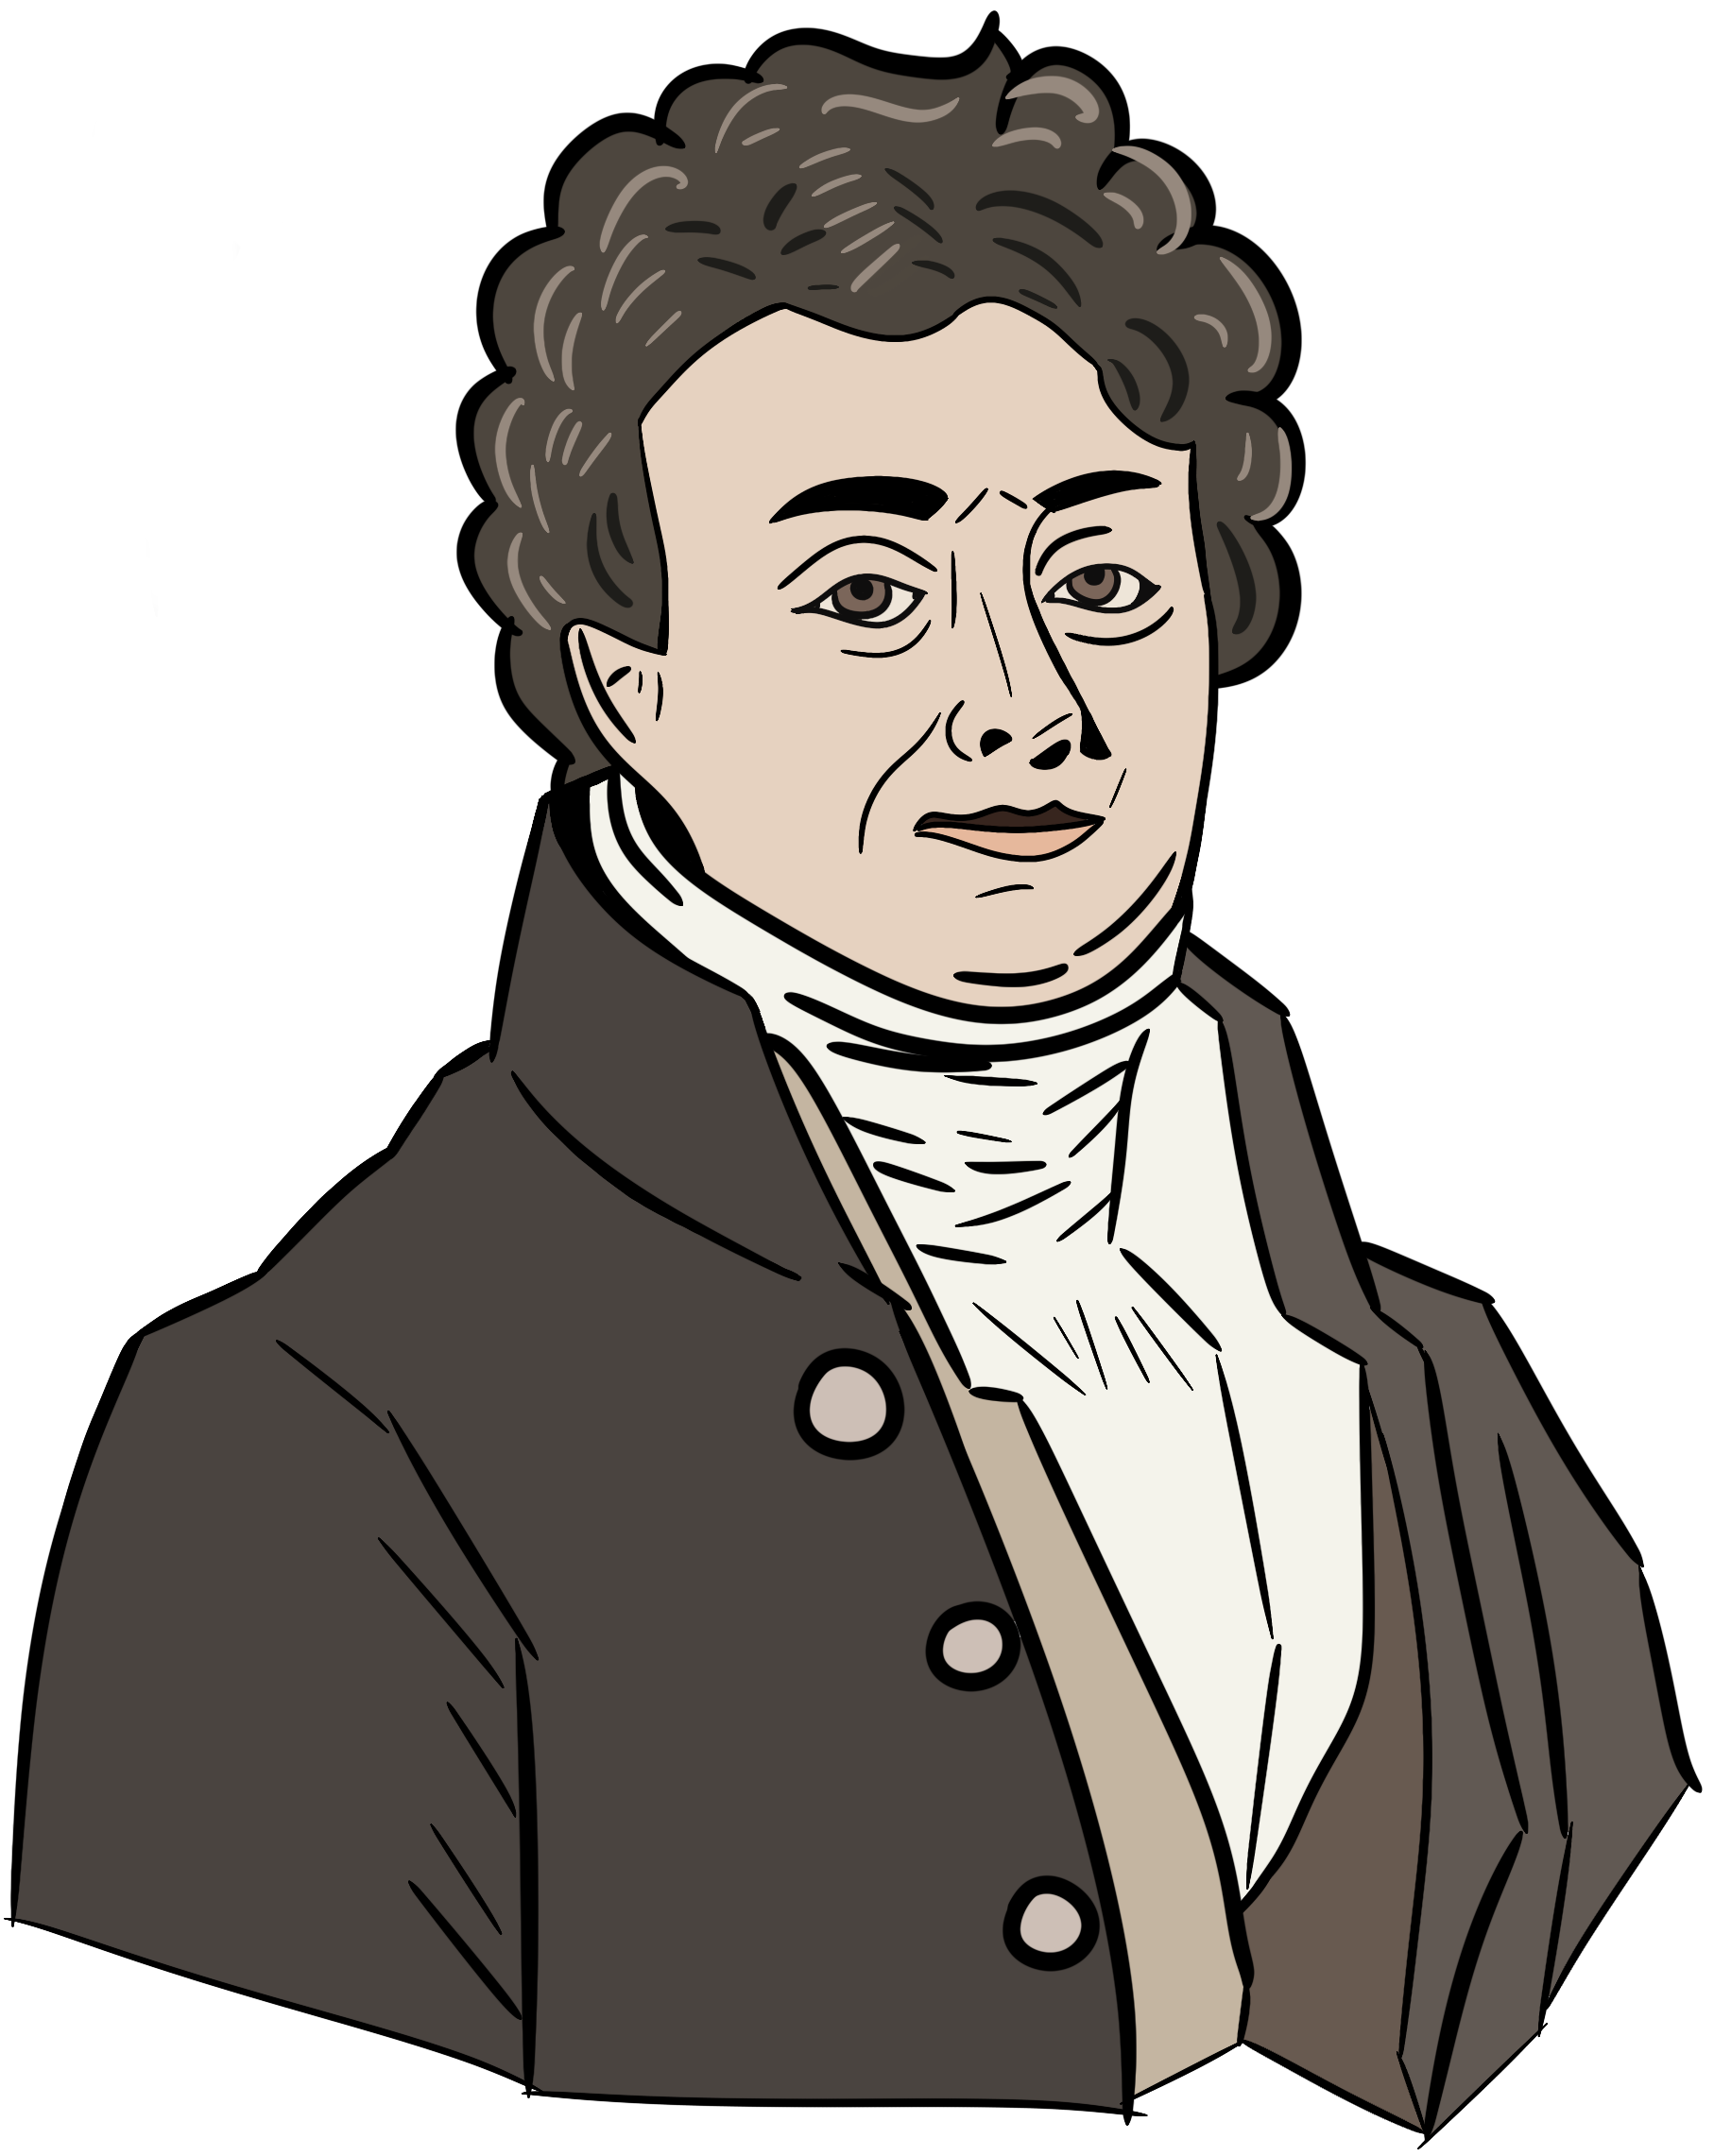
\includegraphics[width=0.5\textwidth]{img/FourierPortrait}
\caption{Jean-Baptiste Joseph Fourier (March 1768 -- May 1830)}
\label{fig:fourier-portrait}
\end{figure}

% ----------------------------------------------------------------------------
% MARK: Panel Layout
% ----------------------------------------------------------------------------

\clearpage
\section{Panel Layout}

% \begin{picture}(0,0)
%   \put(-0.025\paperwidth,-0.38\paperheight){%
%     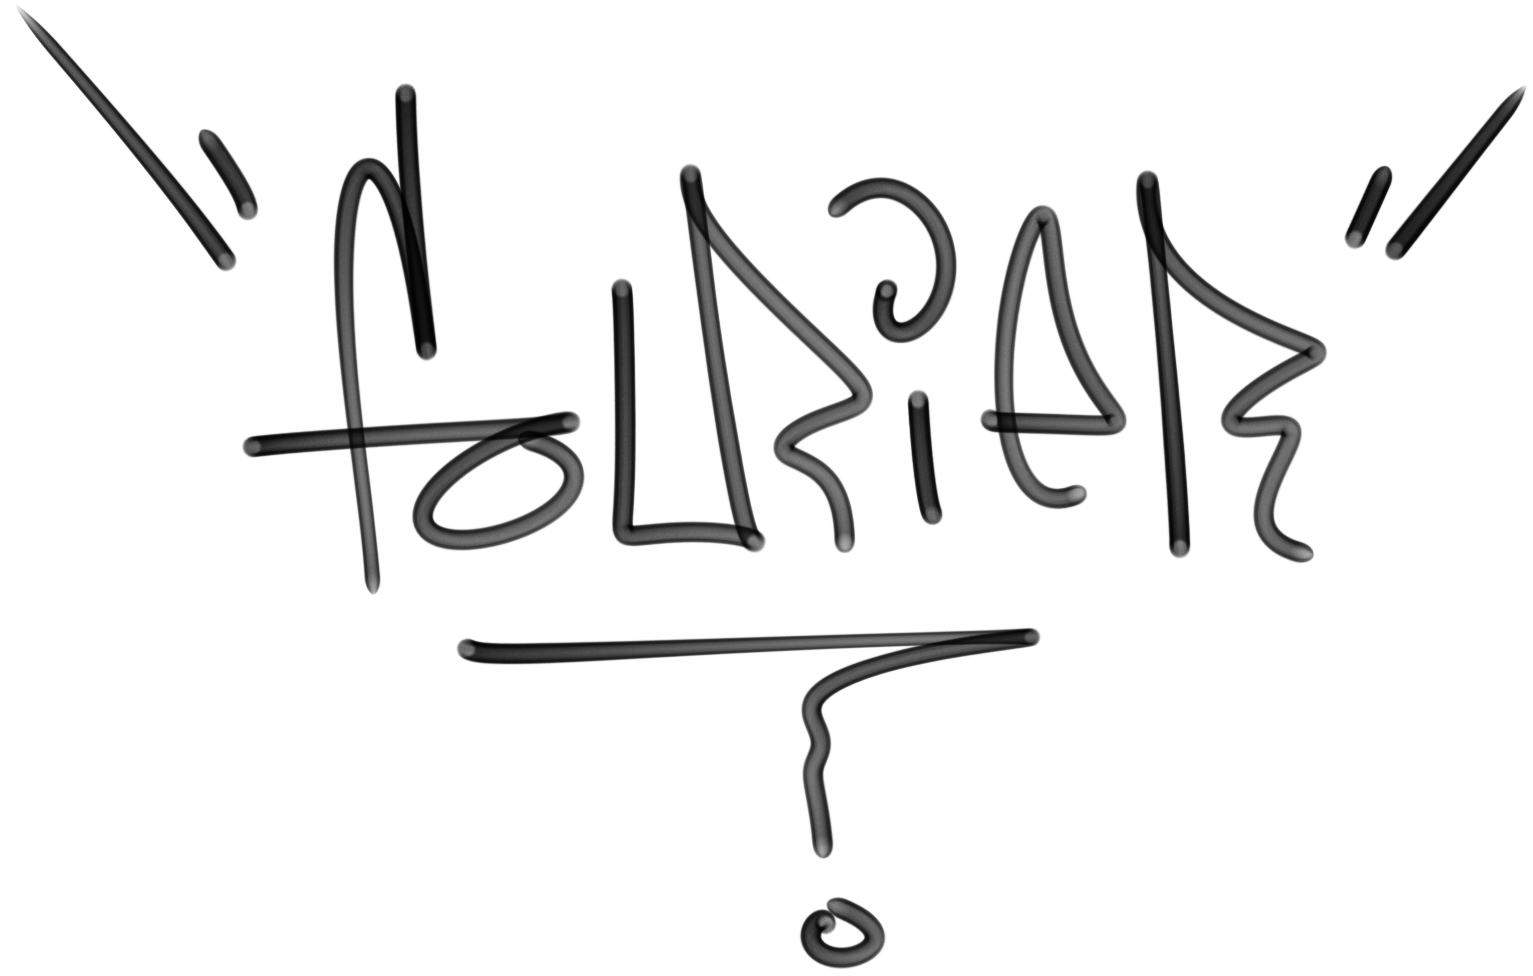
\includegraphics[width=0.15\paperwidth]{img/Tag4}%
%   }
% \end{picture}

\begin{figure}[!htp]
\centering
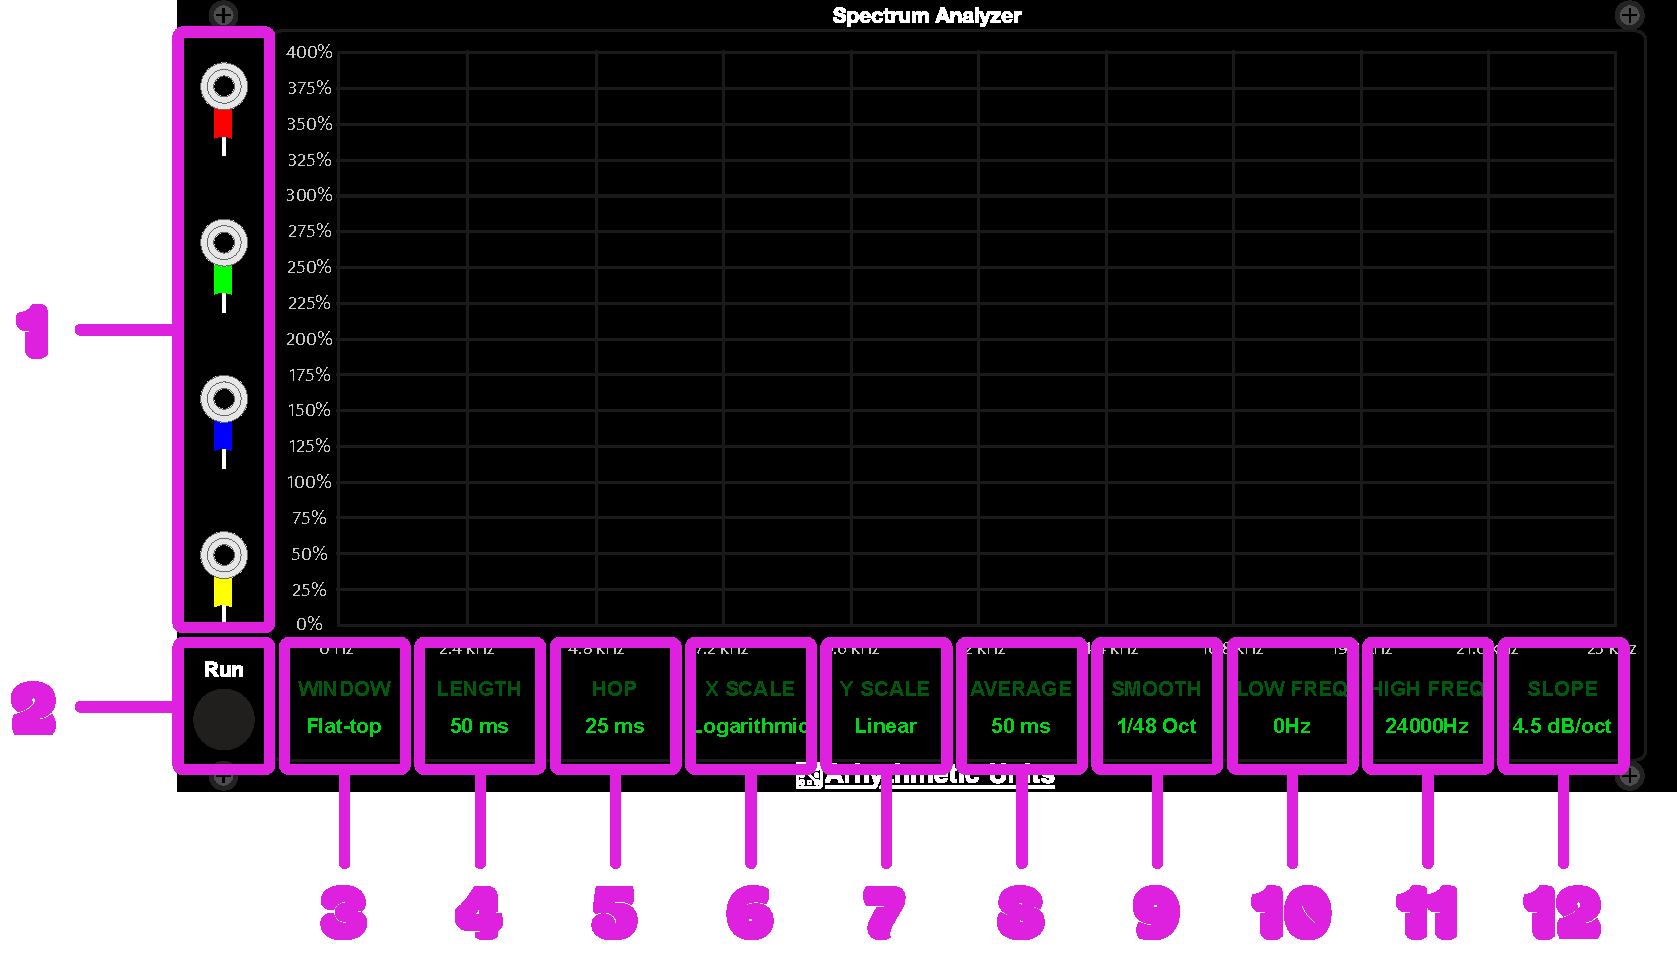
\includegraphics[width=\textwidth]{img/PanelLayout}
\end{figure}

\subsection{Input}

Fourier provides four independent monophonic \textbf{Input} channels. Each
channel features an exponential input gain control ranging from $-\infty\,dB$
(complete silence) to $12\,dB$ (approximately four times the nominal level.)
The channels are color-coded so that each input's panel color matches the
corresponding waveform curve. Fourier’s palette is based on simple primary
colors (with the addition of yellow) to ensure optimal compatibility with
rendering overlays.

\subsection{Run}

The \textbf{Run} button governs the buffering of incoming audio into the
analysis window. When illuminated, Fourier continuously buffers and analyzes
new input samples. When dark, Fourier maintains the display of the current
analysis window without updating it with additional audio frames.

% TODO: This is useful for...
% TODO: Clarify that some parameters may be changed while others not.
% TODO: Maybe we could implement such that you can change parameters while
%       the module is not running? This would require a change to the filter
%       for time smoothing (and maybe increased compute). But, it also leads
%       into the integration of the spectrogram functionality?

\subsection{Window Function}

% \begin{picture}(0,0)
%   \put(\paperwidth - 275,-0.5 \paperheight + 20){%
%     
\includegraphics[width=0.2\paperwidth]{img/Tag8}%
%   }
% \end{picture}

When performing spectral analysis, a phenomenon known as \textit{spectral
leakage} occurs. This effect arises because the analysis is conducted over a
limited time frame while the underlying mathematical framework assumes the
signal repeats infinitely. To minimize these artifacts, the audio input
buffer is typically multiplied by a \textbf{Window Function} that tapers the
sample edges and reduces leakage. Fourier offers a selection of 15 commonly
used window functions, allowing you to balance the trade-off between
frequency resolution and spectral leakage artifacts.

Figure~\ref{fig:window-function-sinusoids} illustrates the impact of
different window functions when analyzing sinusoidal waveform inputs. In
Fig.~\ref{fig:window-function-sinusoids-boxcar}, the Boxcar (i.e.,
rectangular) window is shown; it provides high frequency resolution but also
exhibits significant spectral leakage.
Fig.~\ref{fig:window-function-sinusoids-hamming} demonstrates the effect of a
Hamming window, which trades some frequency resolution for reduced leakage.
Finally, Fig.~\ref{fig:window-function-sinusoids-flattop} displays a Flat-top
window, characterized by low frequency resolution and minimal spectral
leakage.

\begin{figure}[!htp]
\centering
\subfloat[\centering Boxcar Window]{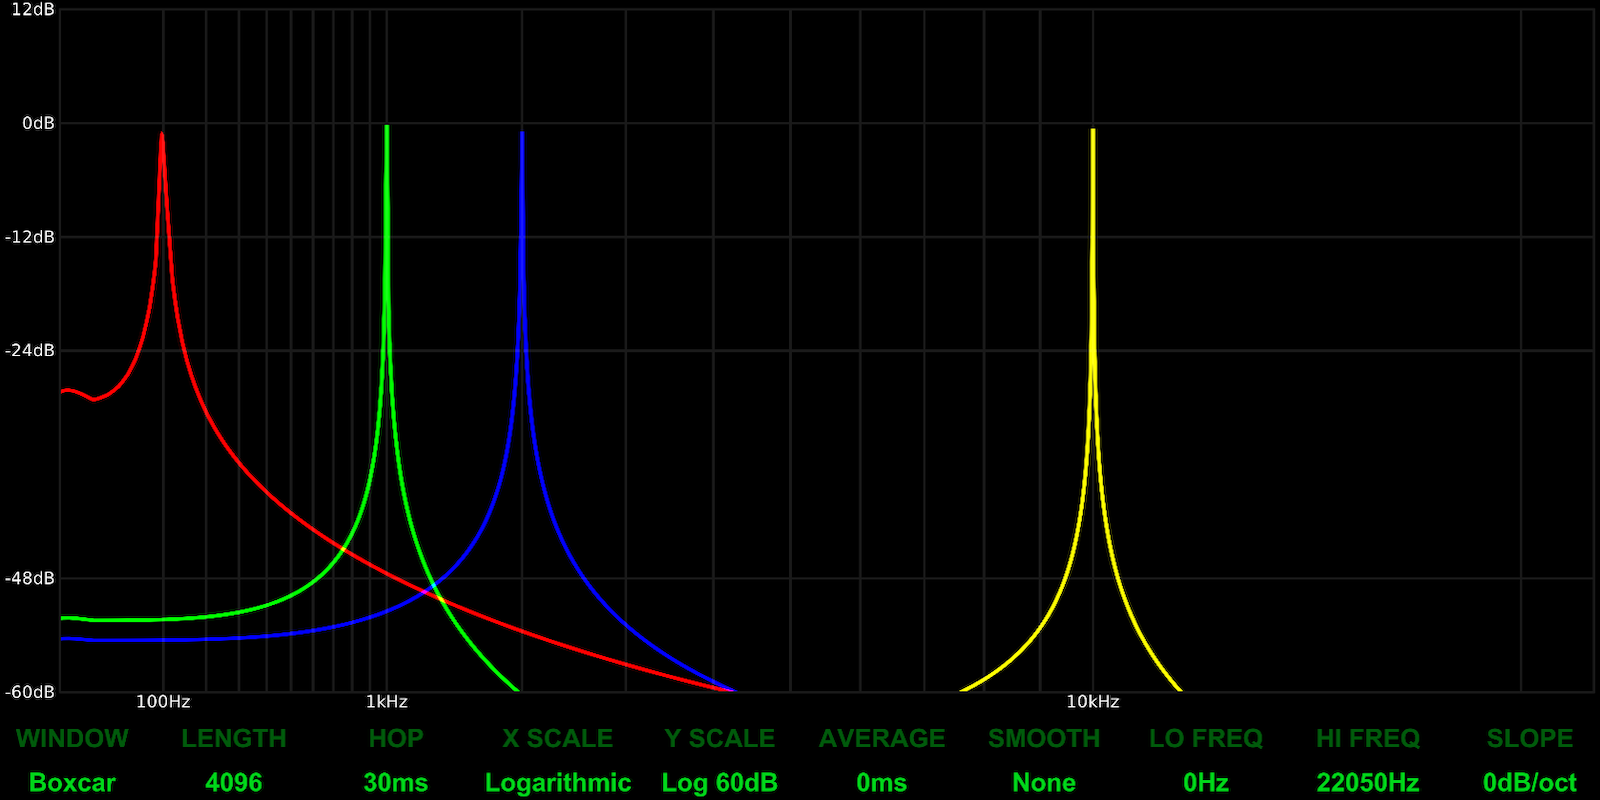
\includegraphics[width=0.33\textwidth]{img/Window/Boxcar}\label{fig:window-function-sinusoids-boxcar}}
\hfill
\subfloat[\centering Hamming Window]{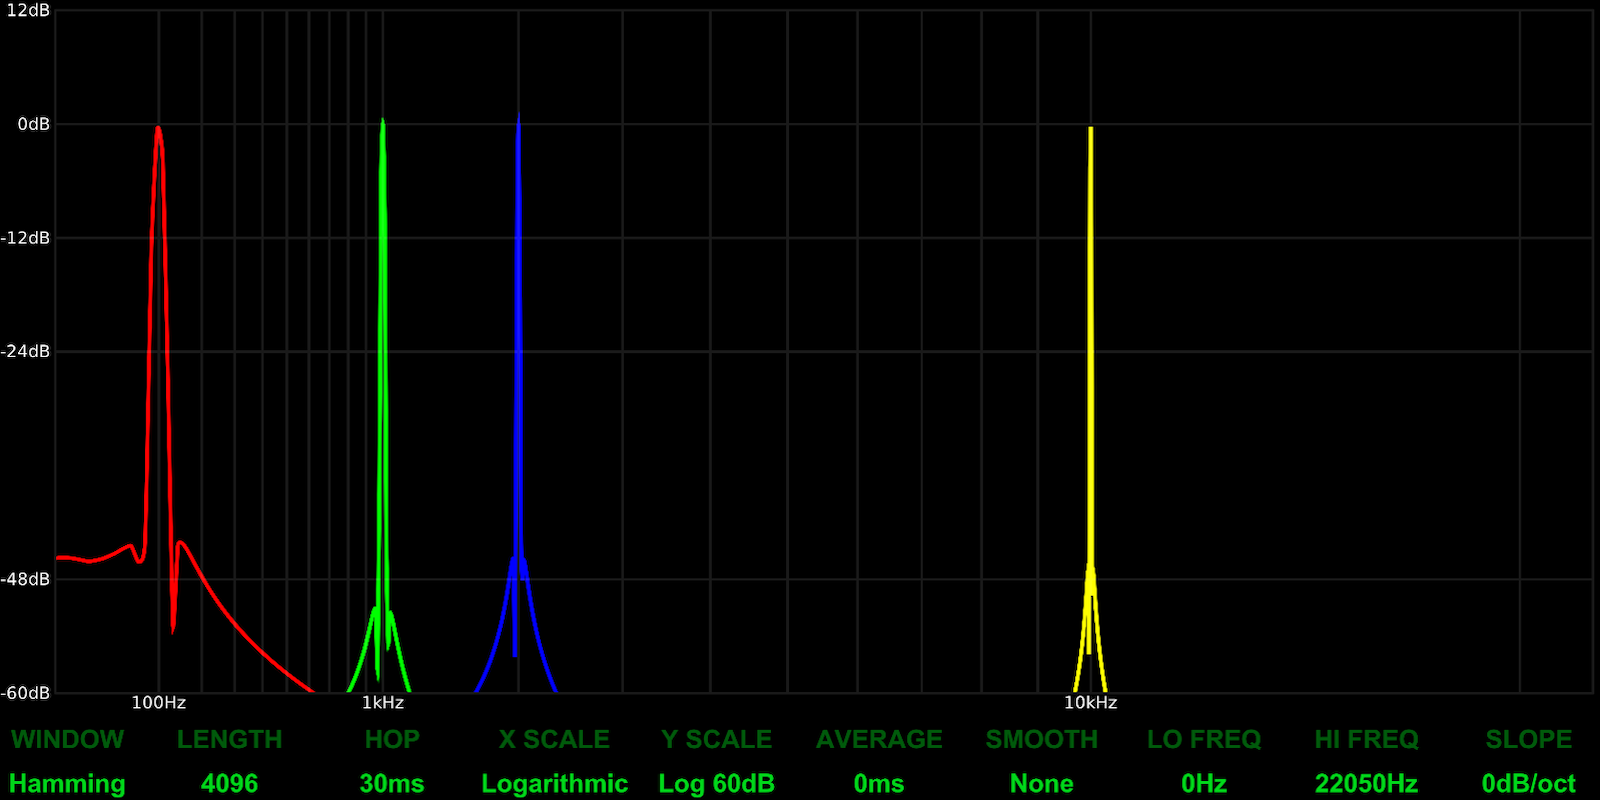
\includegraphics[width=0.33\textwidth]{img/Window/Hamming}\label{fig:window-function-sinusoids-hamming}}
\hfill
\subfloat[\centering Flat-top Window]{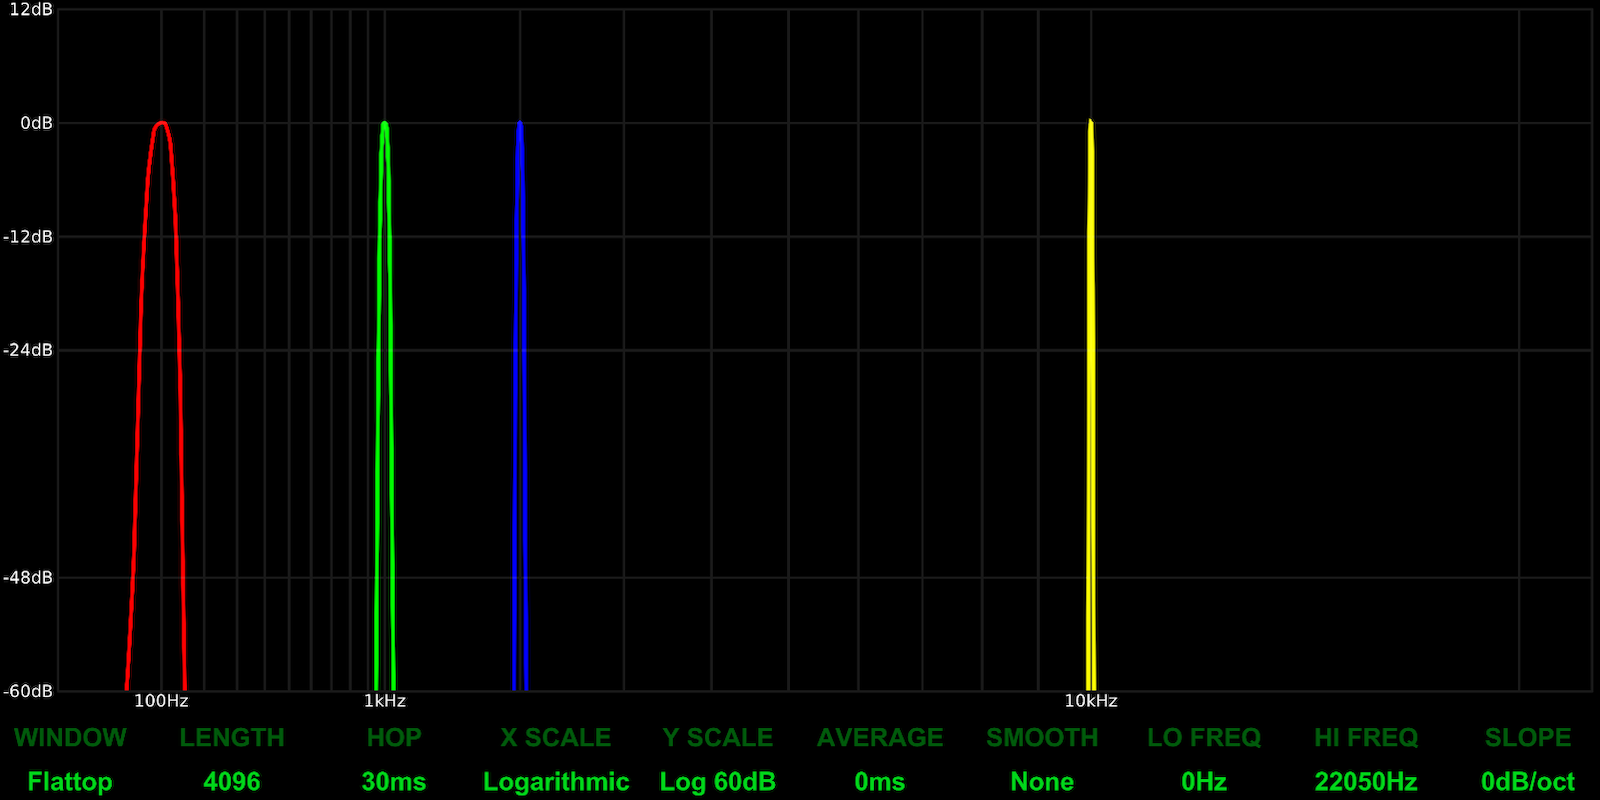
\includegraphics[width=0.33\textwidth]{img/Window/Flattop}\label{fig:window-function-sinusoids-flattop}}
\caption{Sinusoids being analyzed with various window functions.}
\label{fig:window-function-sinusoids}
\end{figure}

\subsection{Length}

The \textbf{Length} parameter sets the size of the audio buffer used for
analysis. Its values follow an exponential series with base $2$, which is
convenient for both musical and computational reasons. Essentially, the
Length parameter defines the resolution of the analysis: longer buffers yield
higher frequency resolution. However, larger values also demand more
processing power. In particular, if the length is represented as an integer
$N$, the computational cost per analysis frame scales as $O(N \log N)$.

Figure~\ref{fig:length-n} illustrates how varying the FFT length parameter
affects the spectral analysis of sinusoidal inputs. In
Fig.~\ref{fig:length-n-1024}, using $N = 2^{10} = 1024$ yields a relatively
coarse frequency resolution, which may be ideal for quick analysis with
minimal computational demand. In contrast, Fig.~\ref{fig:length-n-16384}
shows that a longer FFT length of $N = 2^{14} = 16384$ provides a finer, more
detailed frequency resolution at the expense of increased processing
requirements. Fig.~\ref{fig:length-n-4096} demonstrates an intermediate
setting, offering a balanced trade-off between resolution and computational
load.

\clearpage

\begin{figure}[!htp]
\centering
\subfloat[\centering $N = 2^{10} = 1024$]{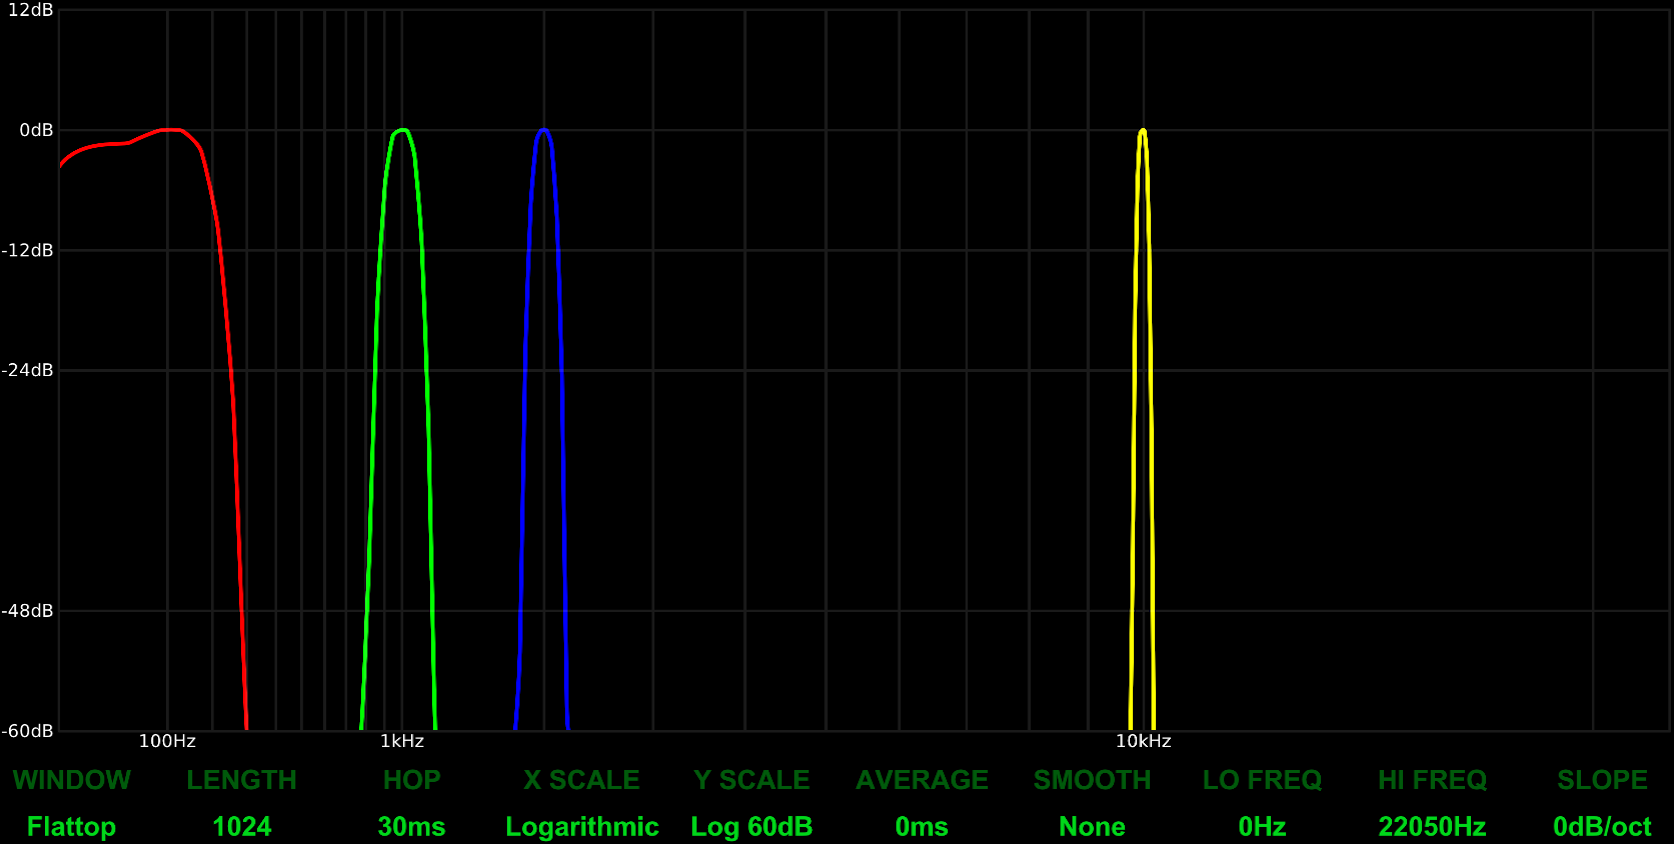
\includegraphics[width=0.33\textwidth]{img/Length/N1024}\label{fig:length-n-1024}}
\hfill
\subfloat[\centering $N = 2^{12} = 4096$]{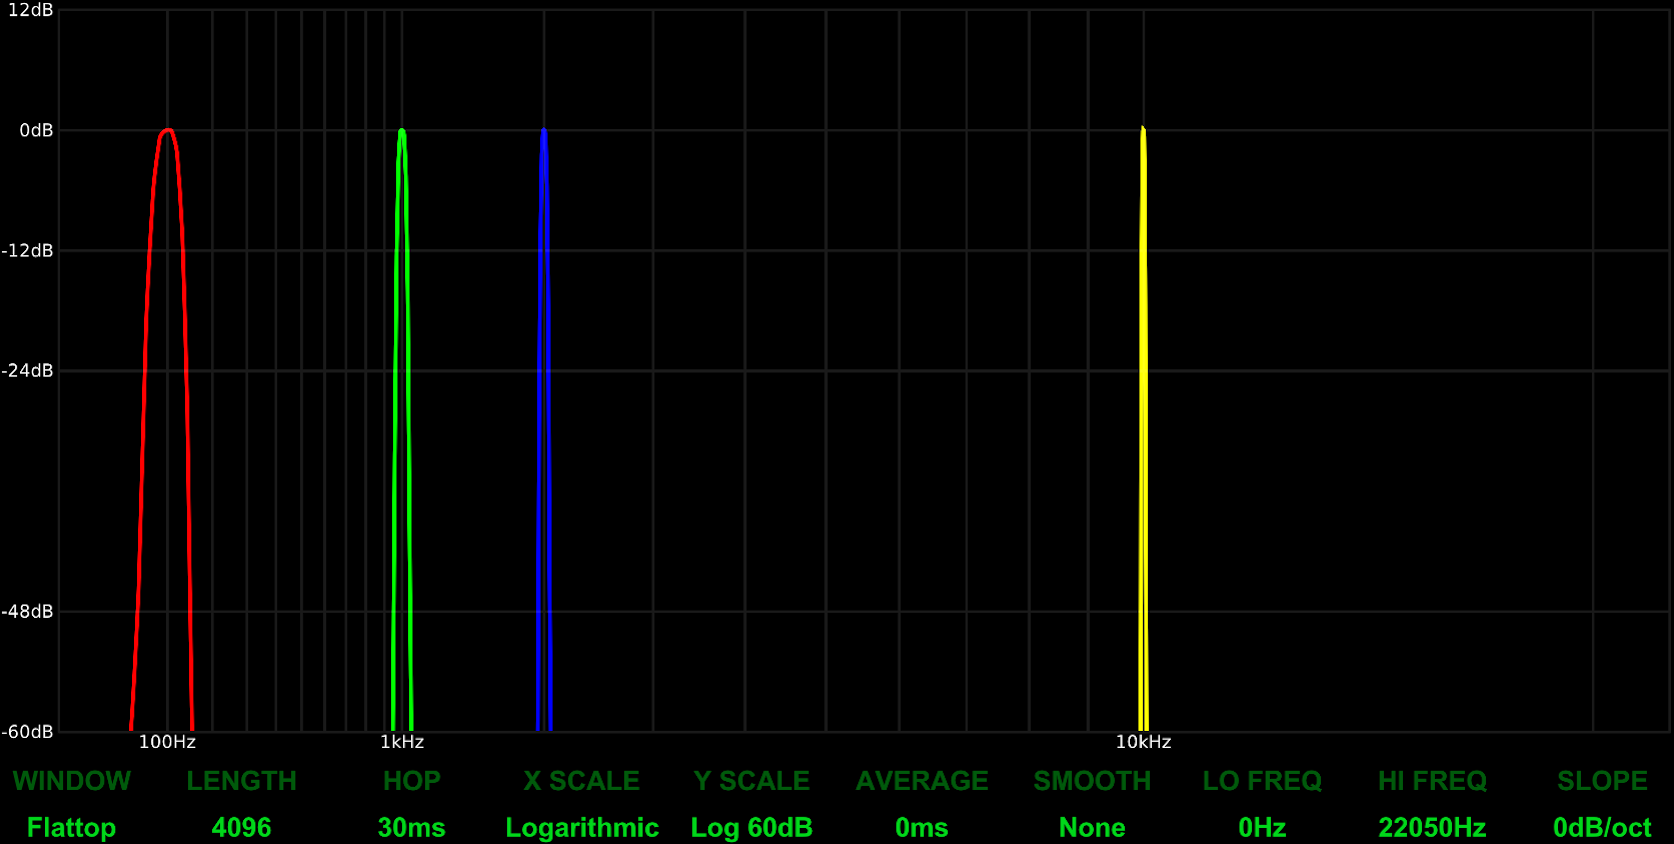
\includegraphics[width=0.33\textwidth]{img/Length/N4096}\label{fig:length-n-4096}}
\hfill
\subfloat[\centering $N = 2^{14} = 16384$]{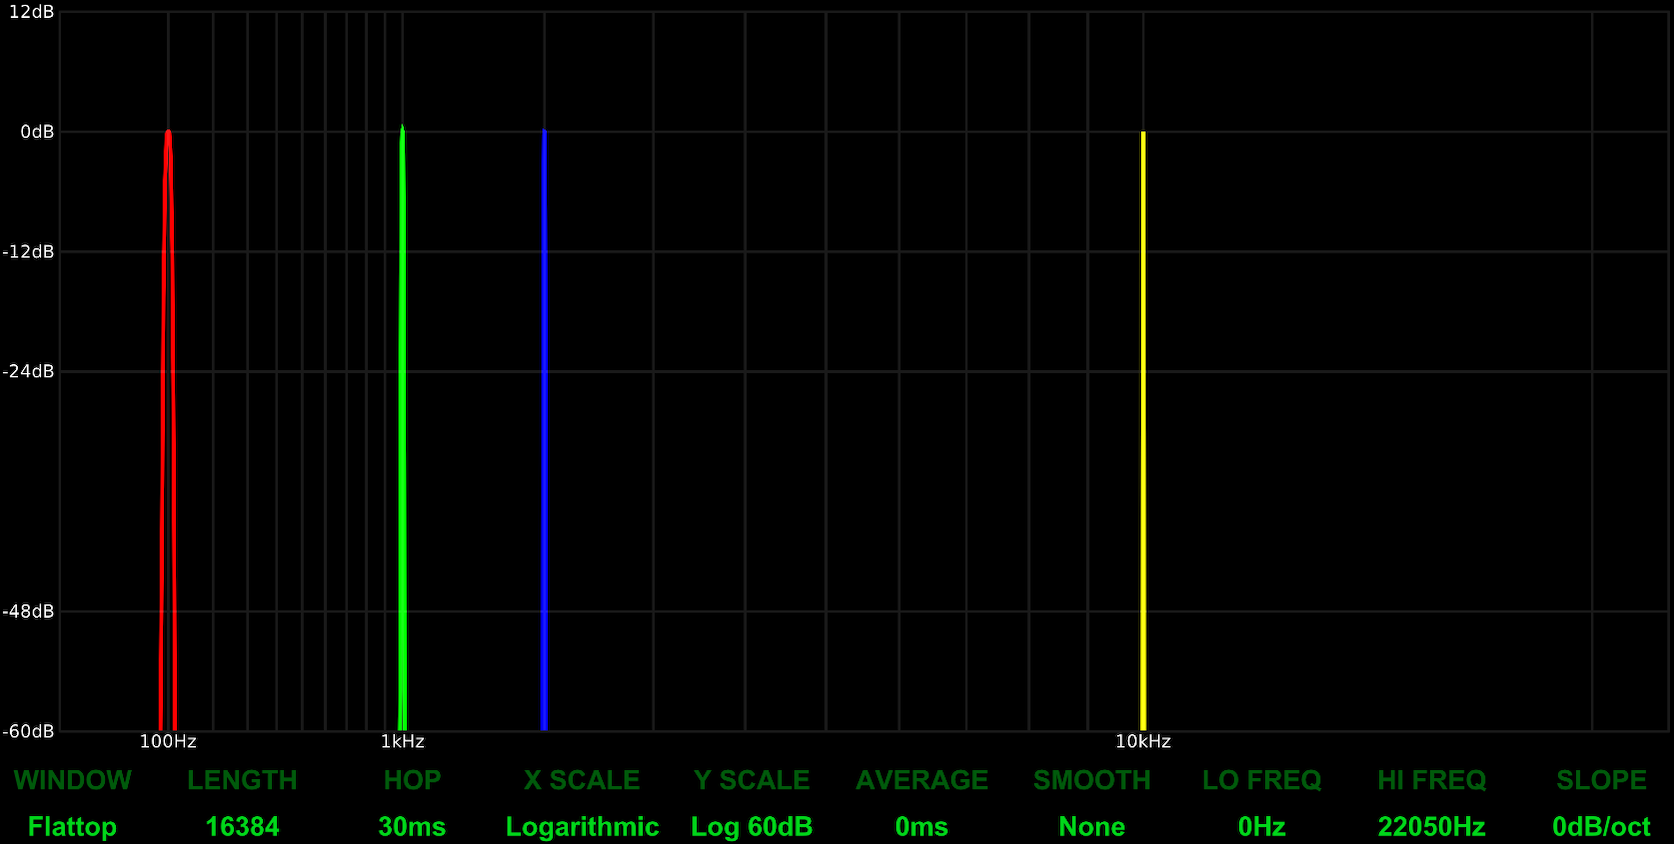
\includegraphics[width=0.33\textwidth]{img/Length/N16384}\label{fig:length-n-16384}}
\caption{Sinusoids being analyzed with various FFT lengths.}
\label{fig:length-n}
\end{figure}

% \begin{picture}(0,0)
%   \put(\paperwidth - 275,-0.1 \paperheight){%
%     
\includegraphics[width=0.2\paperwidth]{img/Tag7}%
%   }
% \end{picture}

\subsection{Hop}

Frequency analysis is performed continuously, providing a real-time
visualization of the live audio feed. The resolution between successive
analysis events is controlled by the \textbf{Hop} rate, which effectively
determines the refresh rate of the module's display.

\subsection{X-Scale}

The \textbf{X-Scale} parameter determines how the frequency bins are
displayed. In \textit{Linear} mode, the frequency bins are evenly spaced,
reflecting the raw, linearly spaced outputs of the Fourier analysis. In
contrast, \textit{Logarithmic} mode arranges the frequency bins on an e
xponential scale, which more closely aligns with human pitch perception.
While the optimal choice depends on the specific frequency patterns you wish
to observe, the Logarithmic setting is typically preferred for its intuitive
representation of pitch.

\subsection{Y-Scale}

The \textbf{Y-Scale} parameter determines how the energy levels of individual
frequency bins are displayed. In \textit{Linear} mode, energy levels are
rendered as percentages ranging from $0\,\%$ to $400\,\%$ of the band's
headroom. In the logarithmic modes, Fourier displays energy levels
exponentially, with ranges set either from $-60\,dB$ or $-120\,dB$ up to
$12\,dB$. As with the X-Scale parameter, the optimal setting for Y-Scale
depends on the aspects of the signal you wish to emphasize, though it is
typically best left in logarithmic mode with a $-60\,dB$ lower limit.

\subsection{Average}

Real-time signal analysis can be noisy, which often obscures the overarching
trends in the signal. The \textbf{Average} parameter adjusts the alpha value
of a 1-pole exponential moving average filter, with its cut-off frequency
expressed in temporal units. This smoothing mechanism allows Fourier to
highlight general frequency trends that align better with human perception.
For musical signal analysis, an averaging time of approximately
$250\,\mathrm{ms}$ is a good starting point.

\subsection{Smooth}

In some cases, frequency analysis can be noisy, particularly when the Length
parameter is set to a large value. To counteract this, the \textbf{Smooth}
parameter applies a smoothing filter to the energy levels of the frequency
analysis bins. This filter is measured in musical octaves, making it
especially suitable for musical analysis. For example, a setting of
$\frac{1}{6}\,Oct$ is a good starting point when using $N \geq 1024$.

\subsection{Low Frequency}

The \textbf{Low Frequency} parameter sets the minimum frequency displayed on
the plot. Adjusting this parameter lets you focus on the lower end of the
frequency spectrum by filtering out any frequencies below the chosen
threshold.

\subsection{High Frequency}

The \textbf{High Frequency} parameter sets the maximum frequency displayed on
the plot. By adjusting this parameter, you can concentrate on higher
frequency content by excluding frequencies above the selected limit.

\subsection{Slope}

The \textbf{Slope} parameter compensates for the natural roll-off of
high-frequency energy in musical signals. For most sound engineering
applications, a slope of either $4.5\,\frac{dB}{Oct}$ or $3\,\frac{dB}{Oct}$
is recommended to enhance the perceptual balance of the frequency spectrum.
Conversely, in engineering applications where a flat frequency response is
desired, a slope of $0\frac{dB}{Oct}$ is typically preferred.

% ----------------------------------------------------------------------------
% MARK: Background
% ----------------------------------------------------------------------------

\clearpage
\section{Background}

Fourier analysis is fundamentally based on the Discrete Fourier Transform
(DFT), which expresses a finite-length signal as a sum of sinusoids with
discrete frequencies. Given an input signal $x[n]$ of length $N$, the DFT
produces a sequence $X[k]$, where the $k$th element represents the amplitude
and phase of a sinusoid with frequency $\frac{k}{N}f_s$, with $f_s$ denoting
the sample rate. The DFT is defined mathematically as:
\begin{equation}
X[k] = \sum_{n=0}^{N-1} x[n] \, e^{-j2\pi k \frac{n}{N}},
\label{eqn:dft}
\end{equation}
for $k = 0, 1, \dots, N-1$. Because the DFT assumes the signal is periodic,
its spectrum is symmetric about the Nyquist frequency
$\left(\frac{f_s}{2}\right)$ and repeats periodically.

\subsection{Windowing Functions}

When analyzing finite-length signals, discontinuities at the boundaries can
introduce \textit{spectral leakage}, where energy from one frequency bin
bleeds into adjacent bins. To mitigate this, a window function is applied to
the signal to taper its edges smoothly. The windowed signal $x_w[n]$ is
obtained by an element-wise multiplication:
\begin{equation}
x_w[n] = x[n] \cdot w[n],
\label{eqn:window}
\end{equation}
where $w[n]$ is the window function. Common choices include the rectangular
(Boxcar), Hann, Hamming, and Blackman windows, each offering a different
balance between frequency resolution (main lobe width) and leakage (side
lobe levels.)

\subsection{Fast Fourier Transform (FFT)}

In practical applications, the DFT is computed efficiently using the Fast
Fourier Transform (FFT) algorithm. One of the most widely used FFT algorithms
is the Cooley-Tukey algorithm, which recursively decomposes the DFT into
smaller DFTs, reducing the computational complexity from $O(N^2)$ to
$O(N \log N)$. Listing~\ref{alg:cooley-tukey} shows a high-level outline of
the \textit{iterative} Cooley-Tukey algorithm, which implements recursion
with loops.

\begin{algorithm}[H]
\SetAlgoLined
\KwIn{Complex array \( x \) of length \( N \) (assume \( N \) is a power of 2)}
\KwOut{The DFT of \( x \)}
\textbf{Bit-Reversal:} Reorder elements of \( x \) according to bit-reversed order of indices\;
\For{\( s \gets 1 \) \KwTo \( \log_2 N \)}{
    \( m \gets 2^s \)\;
    Compute the primitive \( m \)th root of unity: \( W_m \gets e^{-j\frac{2\pi}{m}} \)\;
    \For{\( k \in \{0,\, m,\, 2m,\, \ldots,\, N-m\} \)}{
        \For{\( j \gets 0 \) \KwTo \( \frac{m}{2}-1 \)}{
            \( t \gets W_m^j \cdot x\left[k+j+\frac{m}{2}\right] \)\;
            \( u \gets x[k+j] \)\;
            \( x[k+j] \gets u + t \)\;
            \( x\left[k+j+\frac{m}{2}\right] \gets u - t \)\;
        }
    }
}
\Return \( x \)\;
\caption{Iterative Cooley-Tukey FFT (Simplified)}
\label{alg:cooley-tukey}
\end{algorithm}

This iterative method efficiently computes the FFT by combining the results
of smaller DFTs in a structured manner, greatly reducing the number of
computations required for spectral analysis.

\subsection{Memoization of Twiddle Factors}

In the Cooley-Tukey FFT algorithm, the twiddle factors
\[
W_m^j = e^{-j\frac{2\pi j}{m}},
\]
where \( m = 2^s \) for a given stage \( s \) and
\( j = 0, 1, \ldots, \frac{m}{2}-1 \), are used repeatedly in the butterfly
computations. Since these values depend solely on the stage size \( m \) and
the index \( j \) (and not on the specific input data), they are ideal
candidates for memoization.

Memoization involves precomputing the twiddle factors once and storing them
in a lookup table (or array) during an initialization phase. In practical
implementations, this means:
\begin{itemize}
  \item \textbf{Precomputation:} For each stage \( s \) with block size
  \( m \), compute the \( \frac{m}{2} \) twiddle factors
  \( \{W_m^j\}_{j=0}^{\frac{m}{2}-1} \) before beginning the main FFT
  processing loop.
  \item \textbf{Reuse:} During the FFT computation, instead of recalculating
  \( W_m^j \) for each butterfly operation, the algorithm simply looks up the
  precomputed value. This saves significant computation time, especially for
  large FFT sizes or when processing multiple FFTs of the same length.
  \item \textbf{Efficiency:} By reducing the number of complex exponential
  evaluations (which are computationally expensive), memoization contributes
  to an overall reduction in the algorithm's runtime, making real-time signal
  processing more efficient.
\end{itemize}

While memoization does incur a small memory overhead, the trade-off is
generally favorable in performance-critical applications. In many modern FFT
libraries, such optimizations are implemented by default to accelerate
repeated or real-time spectral analyses.

\subsection{Memoization of Bit-Reversal Table}

In many FFT algorithms, including the iterative Cooley-Tukey method, the input
sequence must first be reordered into bit-reversed order. Since this
permutation depends solely on the FFT length, it can be computed once and
stored in a lookup table. This memoization avoids recalculating the
bit-reversed indices for every new FFT computation, thereby reducing overhead
and speeding up the initialization phase.

For an FFT of length \( N \) (with \( N = 2^r \) for some integer \( r \)),
each index \( i \) in the range \( 0 \leq i < N \) can be expressed in its
binary form:
$$
i = \sum_{k=0}^{r-1} b_k \, 2^k, \quad \text{with } b_k \in \{0,1\}.
$$
The bit-reversed index \( \tilde{i} \) is obtained by reversing the order of
the binary digits:
$$
\tilde{i} = \sum_{k=0}^{r-1} b_k \, 2^{r-1-k}.
$$

This concept can be expressed in pseudo-code by Listing~\ref{alg:bit-reversal}.
In this form, it may be serialized to RAM, disk, or some other persistent
indexing scheme to reduce computational overhead of computing the mapping.

\begin{algorithm}[H]
\SetAlgoLined
\KwIn{FFT length \( N \) (assume \( N = 2^r \) for some integer \( r \))}
\KwOut{Bit-reversal table \( T \) where \( T[i] = \tilde{i} \) for \( i = 0,1,\dots,N-1 \)}
Determine \( r \gets \log_2 N \)\;
\For{\( i \gets 0 \) \KwTo \( N-1 \)}{
    Set \( \tilde{i} \gets 0 \)\;
    Set \( x \gets i \)\;
    \For{\( j \gets 0 \) \KwTo \( r-1 \)}{
        \( \tilde{i} \gets (\tilde{i} \ll 1) \;|\; (x \,\&\, 1) \)\;
        \( x \gets x \gg 1 \)\;
    }
    Set \( T[i] \gets \tilde{i} \)\;
}
\Return \( T \)\;
\caption{Precomputation of the Bit-Reversal Table}
\label{alg:bit-reversal}
\end{algorithm}

\subsection{Real-Valued Fourier Transform (RFFT)}

In musical applications, the input signal is typically purely real-valued.
Because the Fourier transform of a real signal exhibits Hermitian
symmetry -- where negative frequency components mirror the positive ones --
the Real--Valued Fourier Transform (RFFT) can compute only the non-redundant
half of the spectrum. This results in a significant reduction in both
computational complexity and memory usage compared to a full complex FFT. The
RFFT is implemented by packing a real-valued signal of length $N$ into a
complex sequence of length $\frac{N}{2}$ where the real components are
derived from the even--indexed samples and the imaginary components from the
odd--indexed samples. A length $\frac{N}{2}$ FFT is then computed over the
packed signal and reconstructed into DFT coefficients of the $N$-point DFT.

Given a real-valued input signal \( x[n] \) of length \( N \) (with \( N \) a power of 2), the RFFT is computed in three stages:

\paragraph{1. Packing}
The real input is packed into a complex sequence of length \( M = \frac{N}{2} \) by grouping even and odd samples:
\begin{equation}
y[k] = x[2k] + j\,x[2k+1], \quad k = 0, 1, \dots, M-1.
\label{eq:packing}
\end{equation}

\paragraph{2. FFT Computation}
Compute the \( M \)-point FFT of the packed sequence:
\begin{equation}
Y[k] = \sum_{n=0}^{M-1} y[n] \, e^{-j \frac{2\pi}{M} k n}, \quad k = 0, 1, \dots, M-1.
\label{eq:fft-computation}
\end{equation}
(The iterative Cooley–Tukey algorithm, as described previously, may be used here.)

\paragraph{3. Finalization (Reconstruction)}
The full \( N \)-point DFT \( X[k] \) is reconstructed using the symmetry properties of the DFT for real signals. Define the twiddle factors as:
\[
W_N^k = e^{-j\frac{2\pi k}{N}}.
\]
Then, the reconstruction is performed as follows:
\begin{itemize}
  \item For the DC and Nyquist bins:
  \begin{align}
    X[0] &= \Re\{Y[0]\} + \Im\{Y[0]\}, \label{eq:dc}\\[1mm]
    X\left[\frac{N}{2}\right] &= \Re\{Y[0]\} - \Im\{Y[0]\}. \label{eq:nyquist}
  \end{align}
  \item For \( k = 1, 2, \dots, \frac{N}{2}-1 \):
  \begin{equation}
    X[k] = \frac{1}{2}\Big[\, Y[k] + Y^*\Big[\frac{N}{2}-k\Big] - j\,W_N^k\Big( Y[k] - Y^*\Big[\frac{N}{2}-k\Big] \Big)\,\Big],
    \label{eq:finalization}
  \end{equation}
  and, by Hermitian symmetry, the remaining coefficients are given by:
  \[
  X[N-k] = X[k]^*.
  \]
\end{itemize}

Listing~\ref{alg:rfft} provides high-level pseudo code describing the
computation of the RFFT given a real-valued signal as input.

\begin{algorithm}[H]
\SetAlgoLined
\KwIn{Real-valued array \( x[n] \) of length \( N \) (assume \( N \) is a power of 2)}
\KwOut{The \( N \)-point DFT \( X[k] \) for \( k = 0,1,\dots,N-1 \)}
\textbf{Packing:}\\
\For{\( k \gets 0 \) \KwTo \( \frac{N}{2}-1 \)}{
  Compute \( y[k] = x[2k] + j\,x[2k+1] \);
}
\textbf{FFT Computation:}\\
Compute the \( \frac{N}{2} \)-point FFT of \( y[k] \) to obtain \( Y[k] \) \;
(see Algorithm~\ref{alg:cooley-tukey} for the iterative FFT).\\
\textbf{Finalization:}\\
Define \( W_N^k = e^{-j\frac{2\pi k}{N}} \) \;
Set
\[
X[0] = \Re\{Y[0]\} + \Im\{Y[0]\}, \quad X\left[\frac{N}{2}\right] = \Re\{Y[0]\} - \Im\{Y[0]\};
\]
\For{\( k \gets 1 \) \KwTo \( \frac{N}{2}-1 \)}{
  Compute
  \[
  X[k] = \frac{1}{2}\Big[\, Y[k] + Y^*\Big[\frac{N}{2}-k\Big] - j\,W_N^k\Big( Y[k] - Y^*\Big[\frac{N}{2}-k\Big] \Big)\,\Big];
  \]
  Set \( X[N-k] = X[k]^* \);
}
\Return \( X[k] \) for \( k = 0,1,\dots,N-1 \)\;
\caption{Real--Valued FFT via Packing, Complex FFT, and Finalization}
\label{alg:rfft}
\end{algorithm}

\subsection{Short-Time Fourier Transform (STFT)}

For time-varying signals, the Short-Time Fourier Transform (STFT) provides a
way to analyze the frequency content over successive time frames. The STFT
involves applying a window function to successive segments of the signal and
computing the DFT for each segment. It is defined as:
\begin{equation}
X(m, k) = \sum_{n=0}^{N-1} x[n + mH] \, w[n] \, e^{-j2\pi k \frac{n}{N}},
\label{eqn:stft}
\end{equation}
where:
\begin{itemize}
  \item $m$ indexes the time frame,
  \item $H$ is the hop size (i.e., the number of samples by which the window
  is shifted between successive frames), and
  \item $N$ is the window length.
\end{itemize}

\subsection{Pipelining the STFT Computation}

In real-time streaming contexts, the STFT is computed on successive frames of
data separated by a hop size \( H \). Typically, each STFT frame is computed
in its entirety once \( H \) new samples have arrived, which can result in
bursty processing loads. To alleviate this, the computation of each frame can
be pipelined across the \( H \) sample intervals between successive frames.

In a pipelined approach, rather than performing the entire FFT for frame
\( m \) in one burst, the workload is evenly divided and executed
incrementally as each new sample is acquired. This means that when a new
sample is received, a small portion of the FFT computation for the current
frame is processed. Over the course of \( H \) samples, the complete FFT for
frame \( m \) is computed.

This strategy offers several benefits:
\begin{itemize}
  \item \textbf{Smooth Processing Load:} The computational effort is spread
  out over time, preventing large bursts of processing that could otherwise
  lead to latency or jitter.
  \item \textbf{Improved Real-Time Performance:} Incrementally updating the
  FFT ensures that the system can maintain a steady pace of analysis, which
  is critical for live audio processing.
  \item \textbf{Enhanced Responsiveness:} By distributing the workload, the
  system can quickly adapt to changes in the incoming audio, improving the
  responsiveness of the visualization.
\end{itemize}

In practical terms, this pipelining may be implemented by dividing the FFT
computation into \( H \) sub-steps. At each new sample, the algorithm updates
a portion of the FFT, caching intermediate results as needed. When all
\( H \) increments have been processed, the complete FFT for the current
frame is available, and the process repeats for the next frame.

This approach helps ensure that performance trends remain consistent, rather
than exhibiting bursty behavior tied to the hop size \( H \), thereby
optimizing the system for real-time streaming applications.

% ----------------------------------------------------------------------------
% MARK: Copyright seal
% ----------------------------------------------------------------------------

\clearpage
\finalPage

\end{document}
